In Chapter~\ref{chap:isomorphism}, we have seen algorithms to compute
isomorphisms, or inclusions, between pairs of finite fields. Now, we want to
integrate these algorithms in a larger global system with potentially as many
finite fields as we want.
\minitoc

\begin{figure}%[h]
  \centering

    \tikzset{
        dotstyle/.style={circle, inner sep = 1.2pt, outer sep = 4pt, fill =
        gray},
        edgetower/.style={thick},
        edgecomp/.style={thick, lightgray}
          }
          \begin{tikzpicture}[scale=.9]
    \coordinate (T2) at (-2, 0.5);
    \node (Fp) at (0, 0) {$\mathbb{F}_p$};
    \node (Fp2) at ($(Fp) + (T2)$) {$\mathbb{F}_{p^2}$};
    \node (Fp4) at ($(Fp2) + (T2)$) {$\mathbb{F}_{p^4}$};
    \node (Fp2l) at ($(Fp4) + (T2)$) {};% {$\FF_p^{(2)}$};
    % ---------------------
    \coordinate (T3) at (-0.7, 2);
    \node (Fp3) at ($(Fp) + (T3)$) {$\mathbb{F}_{p^3}$};
    \node (Fp9) at ($(Fp3) + (T3)$) {$\mathbb{F}_{p^9}$};
    \node (Fp3l) at ($(Fp9) + (T3)$) {};% {$\FF_p^{(3)}$};
    % ---------------------
    \coordinate (T5) at (0.7, 2);
    \node (Fp5) at ($(Fp) + (T5)$) {$\mathbb{F}_{p^5}$};
    \node (Fp25) at ($(Fp5) + (T5)$) {$\mathbb{F}_{p^{25}}$};
    \node (Fp5l) at ($(Fp25) + (T5)$) {};% {$\FF_p^{(5)}$};
    % ---------------------
    \coordinate (Tl) at (2, .5);
    \node (Fpl) at ($(Fp) + (Tl)$) {$\mathbb{F}_{p^\ell}$};
    \node (Fpl2) at ($(Fpl) + (Tl)$) {$\mathbb{F}_{p^{\ell^2}}$};
    \node (Fpll) at ($(Fpl2) + (Tl)$) {};% {$\FF_p^{(\ell)}$};
    % ---------------------
    \node[dotstyle] (dot1) at ($(Fp2) + (Fp3) - (Fp)$) {};
    \node[dotstyle] (dot2) at ($(Fp4) + (dot1) - (Fp2)$) {};
    \node[dotstyle] (dot3) at ($(Fp2) + (Fp5) - (Fp)$) {};
    \node[dotstyle] (dot4) at ($(Fp3) + (Fp5) - (Fp)$) {};
    \node[dotstyle] (dot5) at ($(Fp3) + (Fpl) - (Fp)$) {};
    \node[dotstyle] (dot6) at ($(Fp5) + (Fpl) - (Fp)$) {};
    \node[dotstyle] (dot7) at ($(Fpl2) + (dot6) - (Fpl)$) {};
    % ---------------------
    \draw
    (Fp)
    edge[edgetower] (Fp2)
    edge[edgetower] (Fp3)
    edge[edgetower] (Fp5)
    edge[edgetower] (Fpl)
    (Fp2)
    edge[edgetower] (Fp4)
    edge[edgecomp] (dot1)
    (Fp4)
    edge[edgetower, dotted] (Fp2l)
    edge[edgecomp] (dot2)
    (dot1)
    edge[edgecomp] (dot2)
    (Fp3)
    edge[edgetower] (Fp9)
    edge[edgecomp] (dot1)
    edge[edgecomp] (dot4)
    (Fp9)
    edge[edgetower, dotted] (Fp3l)
    (Fp5)
    edge[edgetower] (Fp25)
    edge[edgecomp] (dot4)
    edge[edgecomp] (dot6)
    (Fp25)
    edge[edgetower, dotted] (Fp5l)
    (Fpl)
    edge[edgetower] (Fpl2)
    edge[edgecomp] (dot6)
    (Fpl2)
    edge[edgetower, dotted] (Fpll)
    edge[edgecomp] (dot7)
    (dot3)
    edge[edgecomp] (Fp2)
    edge[edgecomp] (Fp5)
    (dot5)
    edge[edgecomp] (Fp3)
    edge[edgecomp] (Fpl)
    (dot6)
    edge[edgecomp] (dot7);
  \end{tikzpicture}
  \caption{Extensions of $\mathbb{F}_p$.}
  \label{fig:alg-closure}
\end{figure}

\clearpage
\section{The compatibility problem}
\label{sec:compatibility-problem}

Now that we know how to go from one finite field $\mathbb{F}_{p^a}$ to another
$\mathbb{F}_{p^b}$, with $p\in\mathbb{N}$ a prime number and
\[
  a\,|\,b
\]
two integers, we would like to be able to manage more than $2$ finite fields
simultaneously. In other words, given a family
\[
  \F=\left\{ \mathbb{F}_{p^{a}}\,|\,a\in E \right\}
\]
for $E$ a subset of $\mathbb{N}\setminus\left\{ 0 \right\}$,
we want to be able to compute an embedding
\[
  \mathbb{F}_{p^a}\emb\mathbb{F}_{p^b}
\]
each time that we have $\mathbb{F}_{p^a}, \mathbb{F}_{p^b}\in\F$ with $a$
dividing $b$. On a pratical point of view, we want to build a computer algebra
system where the users can embed the field they are working with in a bigger
finite field, or conversely if an element is known to belong to a smaller field
than the ambient field, project it to a smaller field. In cryptology and coding
theory, finite fields are ubiquitus, and some algorithms require frequent change
of field. For example, in the
quasi-polynomial algorithm for discrete logarithm in small characteristic by
Granger, Kleinjung and Zumbrägel~\cite{GKZ14}, we have to work with a tower of
finite field extensions, and thus a computer algebra system automatically
dealing with the changes would be very convenient in order to implement their
algorithm. On a theoretical point of view, this leads to the question of the
arithmetic in the algebraic closure of some finite field $\mathbb{F}_p$
\[
  \bar{\mathbb{F}}_p=\bigcup_{j\in\mathbb{N}\setminus\left\{ 0
  \right\}}\mathbb{F}_{p^j}
\]
and its representation on a computer, a question that was for example
investigated in~\cite{DDS14}. 

If we \emph{just} want to be able to compute embeddings between two finite
fields in $\F$ when it makes sense, we can just use one of the algorithms presented
in Chapter~\ref{chap:isomorphism} each time we need it. In fact, we want to
build a data structure $\Lambda$ to represent all the extensions of
$\mathbb{F}_p$ that we need, and additionnal sub-goals might be desirable.
\begin{description}
\item[\emph{Effective embeddings:}] for any pair of extensions
  $k\subset K$ in $\Lambda$, there exists an efficiently computable
  embedding $\phi:k\to K$, and algorithms to evaluate $\phi$ on $k$,
  and the section $\phi^{-1}$ on $K$.
\item[\emph{Compatibility:}] the embeddings are \emph{compatible},
  \ie for any triple $k\subset K\subset L$ in $\Lambda$, and
  embeddings $\phi:k\to K$, $\psi:K\to L$, $\chi:k\to L$ such as shown in
  Figure~\ref{fig:compatibility}, one has
  $\chi=\psi\circ\phi$.
  \begin{figure}[h]
    \centering
    \begin{tikzpicture}
      \node (E) at (0, 0) {$k$};
      \node (F) at (1.5, 1) {$K$};
      \node (G) at (0.5, 2) {$L$};

      \draw[arrow] (E) -- (F);
      \draw[arrow] (E) -- (G);
      \draw[arrow] (F) -- (G);

      \node (f12) at (1, 0.25)
      {$\phi$};
      \node (f13) at (-0.1, 1)
      {$\chi$};
      \node (f23) at (1.4, 1.65)
      {$\psi$};
    \end{tikzpicture}

  \caption{Embeddings between finite fields $k\subset K\subset L$.}
  \label{fig:compatibility}
  \end{figure}
\item[\emph{Incrementality:}] the data associated with an extension
  (\eg its irreducible polynomial, change-of-basis matrices, \dots)
  must be computable efficiently and \emph{incrementally}, \ie 
  adding a new field extension to $\Lambda$ does not require
  recomputing data for all extensions already in $\Lambda$.
\item[\emph{Uniqueness:}] any extension of $\mathbb{F}_{p}$ is determined by an
  irreducible polynomial whose definition only depends on the
  characteristic $p$ and the degree of the extension.
\item[\emph{Generality:}] extensions of $\mathbb{F}_{p}$ can be represented by
  arbitrary irreducible polynomials.
\end{description}
We cannot fulfill all these conditions simultaneously, as
uniqueness and generality are in conflict with each other. One might prefer to
look for uniqueness or generality, depending on the situation, but it would
always be better to have effective embeddings, compatibility and incrementality.
In order to achieve the ``effective embeddings'' condition, we can use the
efficient algorithms presented in Chapter~\ref{chap:isomorphism}. The only
problem is that if we have three finite fields
\[
  k\subset K\subset L
\]
and three embeddings $\phi:k\to K$, $\psi:K\to L$, $\chi:k\to L$, there is no
warranty that the diagram of Figure~\ref{fig:compatibility} commutes, \ie
\[
  \chi = \psi\circ\phi.
\]
If we want to achive compatibility, we have to provide extra-work.
The two constructions presented in Sections~\ref{sec:conway}
and~\ref{sec:bosma-canon-steel} are both solutions oriented towards this goal.
Conway polynomials allow \emph{uniqueness} while Bosma, Cannon and Steel
framework allows \emph{generality}.

\section{Conway polynomials}
\label{sec:conway}

% TODO
% ====
%
% Give a reference for the fact that Conway polynomials always exist?

Conway polynomials~\cite{Parker90, Scheerhorn92} are named after J. H. Conway,
who suggested the idea of working with norm-compatible polynomials when
constructing extension fields. They were introduced by Parker in 1990 and
provide embeddings that are easy to compute.

\begin{defi}[Conway polynomials]
  Let $p\in\mathbb{N}$ be a prime number. The $m$-th \emph{Conway polynomial}
  \[
    C_m\in\mathbb{F}_p[X]
  \]
  is the lexicographically smallest monic irreducible polynomial of degree $m$
  that is also primitive (\ie its roots generate $\mathbb{F}_{p^m}^\times$) and
  norm-compatible, \ie if
  \[
    m\,|\,n
  \]
  we have
  \[
    C_m(X^{\frac{p^n-1}{p^m-1}})\mod C_n = 0.
  \]
\end{defi}
The norm compatibility means that if one takes the norm relatively to the
extension 
\[
  \mathbb{F}_{p^n}/\mathbb{F}_{p^m}
\]
of a root of $C_n$, one obtains a root of $C_m$. This compatibility will allow
us to define compatible embeddings. Let $p\in\mathbb{N}$ be a prime number, $m,
n\in\mathbb{N}$ be two integers such that
\[
  m\,|\,n
\]
and let $C_m, C_n\in\mathbb{F}_{p}[X]$ be the $m$-th and the $n$-th Conway
polynomial. Let 
\[
  k=\mathbb{F}_{p^m}=\mathbb{F}_p(\alpha_m)\cong\mathbb{F}_{p}[X]/(C_m)
\]
and
\[
  K = \mathbb{F}_{p^n}=\mathbb{F}_p(\alpha_n)\cong\mathbb{F}_{p}[X]/(C_n)
\]
with $\alpha_m=\bar X\in k$ and $\alpha_n=\bar X\in K$. Now, we define the
embedding
\[
\begin{array}{cccl}
  \embed{k}{K}:&k&\emb &K\\
  & \alpha_m&\mapsto&(\alpha_n)^{\frac{p^n-1}{p^m-1}}
\end{array}
\]
that sends $\alpha_m$ to $(\alpha_n)^{\frac{p^n-1}{p^m-1}}$, the norm of
$\alpha_n$ relative to $k$. Because this is a field morphism, it is implied that
every polynomial in $\alpha_m$ is sent to the same polynomial in
$(\alpha_m)^{\frac{p^n-1}{p^m-1}}$. That is indeed an embedding because of the
norm-compatibility condition in Conway polynomials. This definition also
provides compatibility thanks to the transitivity of the norm: let
\[
  k\subset K\subset L
\]
three finite fields defined using Conway polynomials, let
\[
  N_{K/k}, N_{L/K}, N_{L/k}
\]
be the respective norms of the extensions
\[
  K/k, L/K, L/k
\]
and
\[
  \embed{k}{K}, \embed{K}{L}, \embed{k}{L}
\]
the corresponding embeddings. Then, for any element $x\in L$, we have
\[
  N_{L/k}(x) = N_{K/k}(N_{L/K}(x)),
\]
and it follows, using the fact that $\embed{K}{L}$ and $N_{K/k}$ commute, that
\[
  \embed{k}{L}=\embed{K}{L}\circ\embed{k}{K}.
\]
Therefore, using Conway polynomials to define all finite field extensions allows
compatibility \emph{a priori}: adding a new extension in the lattice does not
require any computation and the form of the embedding is already known. The
only condition is to define each extension using the Conway polynomial of the
corresponding degree. These polynomial always exist so this is possible,
although the best known algorithm to compute Conway polynomials has exponential
complexity~\cite{HL98}. Because the cost of computing Conway polynomials is
prohibitive, they are often precomputed and tabulated up to a certain degree in
many computer algebra systems. As a result, most computer algebra systems use
Conway polynomial to represent finite fields of small degrees, and switch to
other representations when Conway polynomials are no longer available. This
strategy leads to efficient lattices of compatibly embedded finite fields, at
least in small degrees, but at the cost of generality, because the finite fields
extensions cannot be user-defined and high degree extensions cannot be included
in the lattice. We see in Section~\ref{sec:bosma-canon-steel} that those issues
can be adressed by using an other method 
defined by Bosma, Canon, and Steel~\cite{BCS97}, but the price to compute each
embedding is higher.

\section{Bosma-Canon-Steel framework}
\label{sec:bosma-canon-steel}

In 1987, Bosma, Canon and Steel proposed a new framework~\cite{BCS97} to deal
with lattices of finite field extensions. These algorithms were initially
implemented in the computer algebra system MAGMA. The framework allows the user
to define finite fields with custom polynomials, and compute the
correct embeddings on the fly, in a way that guarantees that at least one
compatible embedding will always exist between two finite fields, when that
makes sense. To the best of my knowledge, this framework was only used in MAGMA
until very recently. We first implemented the framework using Nemo and Flint and
presented our software in the symbolic computation conference ISSAC in
2018~\cite{DRR18}. In 2019, the code was also added to the official branch of
Nemo, and Nemo can now deal with finite field extensions and compatibly embed
them, in the case where the characteristic $p$ of the fields fit in a machine
word. There are no theretical obstacles preventing from implementing the algorithm in arbitrary
large characteristic, but some tools were lacking at the C level (\ie in
Flint).

\subsection{Bosma-Canon-Steel algorithm}
\paragraph{Notations and first results.} Let $p\in\mathbb{N}$ be a prime number
and $q$ a power of $p$. We present the results over the finite field
$\mathbb{F}_q$, even if the applications we have in mind apply to prime field
extensions. Given two finite fields $k$ and $K$ with cardinalities
\[
  \Card k = q^m
\]
and
\[
  \Card K =  q^n
\]
such that $m$ divides $n$, we know that $k$ can be embedded in $K$. In other
words, we know that $K$ contains one subfield
\[
  k'=\left\{ x\in K\,|\,x^{q^m}=x \right\}\subset K
\]
with 
\[
  \Card k' = q^m.
\]
There is exactly one subfield $k'$ in $K$ that has the same cardinality as $k$,
but there exist $m$ different ways to map $k$ to $k'$. One way of seeing that is
to say that an element $\alpha\in k$ generating $k$ has a minimal polynomial
$\pi$ over $\mathbb{F}_q$ of degree $m$, and that $\alpha$ can be mapped to any
one of the $m$ roots of $\pi$ in $K$. This choice sets the embedding because any
element in $k$ can be written as
\[
  \sum_{j=0}^{m-1}a_j \alpha^j,
\]
with $a_j\in\mathbb{F}_q$. We write $k\emb K$ if an explicit embedding has been
chosen. Let
\[
  k\subset K\subset L
\]
with $k\emb K$ and $k\emb L$, as in Figure~\ref{fig:uncomplete}. The fundations
of Bosma-Canon-Steel framework lay on the fact that we precisely know how many
compatible embeddings from $K$ to $L$ we can find.
  \begin{figure}%[h]
    \centering
    \begin{tikzpicture}
      \node (E) at (0, 0) {$k$};
      \node (F) at (1.5, 1) {$K$};
      \node (G) at (0.5, 2) {$L$};

      \draw[arrow] (E) -- (F);
      \draw[arrow] (E) -- (G);
      \draw[dashed-arrow] (F) -- (G);

      \node (f12) at (1, 0.25) {$\phi$};
      \node (f13) at (-0.1, 1) {$\chi$};
      %\node (f23) at (1.4, 1.65) {$\psi$};
    \end{tikzpicture}
  \caption{Uncomplete embedding diagram.}
  \label{fig:uncomplete}
  \end{figure}
  \begin{prop}[{\cite[Thm.~2.1]{BCS97}}]
    \label{prop:number-embeddings}
    Let $l\,|\,m\,|\,n$ three integers and
    \[
      k\subset K\subset L
    \]
    three finite fields extensions of $\mathbb{F}_q$, with respective
    cardinalities $q^l$, $q^m$ and $q^n$. Assume that $k\emb K$ and $k\emb L$,
    then there are $m/l$ compatible embeddings from $K$ to $L$.
  \end{prop}
  \begin{proof}
    Let $\phi:k\to K$ be the embedding from $k$ to $K$ and $\chi:k\to L$ the
    embedding from $k$ to $L$. Let $\widetilde\psi:K\to L$ be any embedding from $K$ to
    $L$. The maps $\chi$ and $\widetilde\psi\circ\phi$ are two embeddings from
    $k$ to $L$. Since there are only $l$ such maps, and since the difference
    between them is only a matter of which conjugate is chosen for a generating
    element in $k$, we know that there exist
    \[
      \sigma\in\Gal(L/\mathbb{F}_q)
    \]
    such that
    \[
      \chi = \sigma\circ\widetilde\psi\circ\phi.
    \]
    If we set
    \[
      \psi=\sigma\circ\widetilde\psi,
    \]
    we obtain a compatible embedding $\psi:K\to L$ from $K$ to $L$. If we
    compose $\psi$ with a $\chi(k)$-automorphism of $L$, \ie an automorphism of
    $\psi(K)$ that
    fixes the subfield $\chi(k)$, we still obtain a compatible embedding because
    the images of the elements in $\chi(k)$ are unchanged. Now, we know that
    \[
      \Card\Gal(\psi(K)/\chi(k)) = m/l,
    \]
    thus we know that there are exactly $m/l$ embeddings from $K$ to $L$ that
    are compatible with $\phi$ and $\chi$.
  \end{proof}
  In the future, if we have two finite fields $k$ and $K$ such that $k\emb K$
  with an explicit embedding $\phi:k\to K$, we will often identify $k$ with
  its isomorphic image $\phi(k)\cong k$ in $K$, for the sake of simplicity. We
  also have a constructive version of Proposition~\ref{prop:number-embeddings}.
\begin{prop}[{\cite[Thm.~2.2]{BCS97}}]
    \label{prop:number-embeddings-constructive}
    Let $l\,|\,m\,|\,n$ three integers and
    \[
      k\subset K\subset L
    \]
    three finite fields extensions of $\mathbb{F}_q$, with respective
    cardinalities $q^l$, $q^m$ and $q^n$. Assume that $k\emb K$ and $k\emb L$,
    and let $\phi=\embed{k}{K}$, $\chi=\embed{k}{L}$ the respective embeddings.
    Let also $\alpha\in K$ be an element that generates $K$ over $k$ and
    \[
      \pi_k=\Minpoly_k(\alpha)
    \]
    the minimum polynomial of $\alpha$ over $k$. Let $\rho\in L$ be a root of
    $\pi_k$ in $L$. Let $\psi:K\to L$ be the map defined by
    \[
      \psi(\sum_{j=0}^{m/l-1}x_j\alpha^j) = \sum_{j=0}^{m/l}x_j\rho^j,
    \]
    using the unique representation of any element of $K$ as $\sum_j x_j
    \alpha^j$ with $x_j\in k$. Then $\psi$ is an embedding from $K$ to $L$ that
    is compatible with $\phi$ and $\chi$, \ie we have
    \[
      \chi = \psi\circ\phi.
    \]
  \end{prop}
  \begin{proof}
    The root $\rho$ in $L$ exists since we know that $\pi_k$ has a root in $K$
    and $K\subset L$. The map $\psi$ is then well-defined because of the uniqueness of the
    representation of the elements in $K$ as $\sum_jx_j\alpha^j$. The elements
    $\alpha$ and $\rho$ have the same minimum polynomial so the map $\psi$ is a
    homomorphism. The map $\psi$ is also injective and thus it is an embedding
    from $K$ to $L$. The compatibility condition holds by construction.
  \end{proof}
  \begin{rem}
    \label{rem:base-field}
   % TODO
   % ====
   %
   % Write something clearer.
   In fact, in our implementation and even in
   Proposition~\ref{prop:several-subfields}, this result will not be used as is and
   we will usually take $\alpha\in K$ and element generating $K$ over the base
   field $\mathbb{F}_q$ instead of over $k$. Indeed, if $\alpha$ generates $K$
   over $\mathbb{F}_q$, it also generates $K$ over $k$. We can still take a root
   $\rho$ of $\Minpoly_{k}(\alpha)$ because
   \[
     \Minpoly_k(\alpha)\,|\,\Minpoly_{\mathbb{F}_q}(\alpha)
   \]
   and so a root of $\Minpoly_{k}(\alpha)$ is \emph{a fortiori} a root of
   $\Minpoly_{\mathbb{F}_q}(\alpha)$. As a result, we can use the
   $\mathbb{F}_q$-algebra structure of $K$ and still achieve compatibility with
   the subfield $k$.
  \end{rem}
  Although the result of Proposition~\ref{prop:number-embeddings} captures only
  one configuration among the three different possibilities of
  Figure~\ref{fig:triangles}, it is the most important case. Indeed, if we
  already know $\embed{k}{K}$ and $\embed{K}{L}$ (the configuration in the
  middle of Figure~\ref{fig:triangles}), we can just set
  \[
    \embed{k}{L} = \embed{K}{L}\circ\embed{k}{K}.
  \]
  Finally the configuration on the right, where we know $\embed{k}{L}$ and
  $\embed{K}{L}$, is also unrelevant because, by construction, this case never
  happens when working with Bosma-Canon-Steel framework.
    \begin{figure}
    \centering
    \begin{tikzpicture}
      \node (E) at (0, 0) {$k$};
      \node (F) at (1.5, 1) {$K$};
      \node (G) at (0.5, 2) {$L$};

      \draw[arrow] (E) -- (F);
      \draw[arrow] (E) -- (G);
      \draw[dashed-arrow] (F) -- (G);
    \end{tikzpicture}
    \phantom{and}
    \begin{tikzpicture}
      \node (E) at (0, 0) {$k$};
      \node (F) at (1.5, 1) {$K$};
      \node (G) at (0.5, 2) {$L$};

      \draw[arrow] (E) -- (F);
      \draw[dashed-arrow] (E) -- (G);
      \draw[arrow] (F) -- (G);

    \end{tikzpicture}
    \phantom{and}
    \begin{tikzpicture}
      \node (E) at (0, 0) {$k$};
      \node (F) at (1.5, 1) {$K$};
      \node (G) at (0.5, 2) {$L$};

      \draw[dashed-arrow] (E) -- (F);
      \draw[arrow] (E) -- (G);
      \draw[arrow] (F) -- (G);

    \end{tikzpicture}
    \caption{The different configurations with triangles.}
    \label{fig:triangles}
  \end{figure}

\paragraph{Description of the framework.} The general strategy of Bosma, Canon,
and Steel to compute and maintain the data of several finite fields and
compatible embeddings between them is to ensure that some properties are
conserved at all times. In all the section, we fix $p\in\mathbb{N}$ a prime
number and $q$ a power of $p$. The results are true for an arbitrary power of
$p$, although the applications and the implementations we have in mind are
relevant for $q=p$. If $k=\mathbb{F}_{q^m}$ is a finite extension of
$\mathbb{F}_q$, we define
\[
  \partial (k) = \left[ k:\mathbb{F}_q \right] = m
\]
the extension degree over $\mathbb{F}_q$.
\begin{defi}[Lattice of compatibly embedded finite fields]
  \label{defi:lattice-bcs}
  Let $q$ be a power of $p$ a prime number and $\mathbb{F}_q$ the finite field
  with $q$ elements. The couple
\[
  \Lambda = (\mathcal K, \Phi),
\]
where $\mathcal K$ is a collection of finite fields sharing the same base field
$\mathbb{F}_q$ and $\Phi$ is a collection of embeddings between members of
$\mathcal K$,
is called a \emph{lattice of compatibly embedded finite fields} if the following
conditions are satisfied:
\begin{description}
  \item[CE1 (unicity)] for each pair $(k, K)$ of elements in $\mathcal K$, there exists
    at most one corresponding embedding $\embed{k}{K}\in\Phi$.
    \item[CE2 (reflexivity)] For each $k\in \mathcal K$, the identity map
    $\Id_k=\embed{k}{k}$ is in $\Phi$.
  \item[CE3 (base subfield)] There is exactly one $k\in \mathcal K$ such that
    $\partial(k)=1$, and for all $K\in \mathcal K$, there exists $\embed{\mathbb{F}_q}{K}\in\Phi$.
  \item[CE4 (invertibility)] If $k\emb K$ and $\partial(k)=\partial(K)$, then $K\emb k$ and
    $\embed{K}{k}=\embed{k}{K}^{-1}$.
  \item[CE5 (transitivity)] For any triple $(k, K, L)$ of elements in $\mathcal
    K$, if $E\emb F\emb G$ then $E\emb G$ and
    $\embed{E}{G}=\embed{F}{G}\circ\embed{E}{F}$.
  \item[CE6 (intersections)] For each $k, K, L\in \mathcal K$ such that $K\emb L$ and
    $k\emb L$, there exists $I\in \mathcal K$ such that
    $\partial(I)=\gcd(\partial(k), \partial(K))$
    and $I\emb k$, $I\emb K$.
\end{description}
\end{defi}
Conditions CE1 to CE5 are quite natural, some of them are technical and
are not important in our implementation. For example, Condition~CE3
is totally free in our implementation because we work with $q=p$ and the
elements of our fields are represented by polynomials over
$\mathbb{F}_p=\mathbb{Z}/p\mathbb{Z}$, thus the subfield
$\mathbb{F}_p\subset\mathbb{F}_{p^m}$ is always represented by the constant
polynomials and the embedding is trivial. Nevertheless, Condition~CE6 is
important both on a theoretical and on an implementation point of view: it
ensures that the implicit embeddings between common subfields are made explicit,
in order to prevent any possible future incompatibility, and it forces the
computer algebra software to compute extra embeddings that the user might not
need. Assume that we have embedded $\mathbb{F}_{p^4}$ and $\mathbb{F}_{p^6}$
into $\mathbb{F}_{p^{12}}$, there is now an implicit isomorphism between the two
copies of the quadratic subfield $\mathbb{F}_{p^2}$ in $\mathbb{F}_{p^4}$ and
$\mathbb{F}_{p^6}$. Any future embedding from $\mathbb{F}_{p^4}$ of
$\mathbb{F}_{p^6}$ in an extension of
$\mathbb{F}_{p^{12}}$, say $\mathbb{F}_{p^{24}}$ for example, must now take into
account the isomorphism between the two quadratic fields. Condition CE6 ensures
that this implicit isomorphism is made explicit by adding a quadratic field
$\mathbb{F}_{p^2}$ in the lattice and explicitly embedding it in
$\mathbb{F}_{p^4}$ and $\mathbb{F}_{p^6}$, and by transitivity in
$\mathbb{F}_{p^{12}}$ and $\mathbb{F}_{p^{24}}$.
\begin{center}
      \begin{tikzpicture}
        \node (4) at (0, 0) {$\mathbb{F}_{p^{4}}$};
        \node (6) at (2, 0) {$\mathbb{F}_{p^{6}}$};
        \node (12) at (1, 2) {$\mathbb{F}_{p^{12}}$};
        \node (24) at (1, 4) {$\mathbb{F}_{p^{24}}$};

      \draw[arrow] (4) -- (12);
      \draw[arrow] (6) -- (12);

      \node[rotate=90] (sub1) at (0, -0.5) {$\subset$};
      \node[rotate=90] (sub2) at (2, -0.5) {$\subset$};
        \node (2) at (0, -1) {$\mathbb{F}_{p^{2}}$};
        \node (2bis) at (2, -1) {$\mathbb{F}_{p^{2}}$};
        \node (iso) at (1, -1) {$\cong$};
      \draw[dashed-arrow] (12) -- (24);
      \draw[dashed-arrow] (4) to[bend left] (24);
      \draw[dashed-arrow] (6) to[bend right] (24);
    \end{tikzpicture}
\end{center}
Under the conditions described in Definition~\ref{defi:lattice-bcs}, we
can add new embeddings in our lattice $\Lambda$ without compromising the
compatibility of the lattice. Assume that we want to embed $K$ into $L$. We have
seen that the relevant elements that restrict the number of compatible
embeddings are the common subfields of $K$ and $L$. If there is only one common
subfield $k$, we are in the case described by
Propositions~\ref{prop:number-embeddings}
and~\ref{prop:number-embeddings-constructive}. Now, assume that there are many
common subfields, like shown in Figure~\ref{fig:uncomplete-sev}.% and let
%\[
%  C = \left\{ k\in\mathcal K\,|\,k\emb K\text{ and }k\emb L \right\}
%\]
%be the set of these common subfields.
\begin{figure}
  \centering
    \begin{tikzpicture}
      \node (E1) at (-2, 0) {$k_1$};
      \node (E2) at (-1, 0) {$k_2$};
      \node (Er) at (0.75, 0) {$k_r$};
      \node (F) at (1.5, 1) {$K$};
      \node (G) at (0.5, 2) {$L$};
      \node (p) at (0, 0) {$\dots$};

      \draw[arrow] (E1) -- (F);
      \draw[arrow] (E1) -- (G);
      \draw[arrow] (E2) -- (F);
      \draw[arrow] (E2) -- (G);
      \draw[arrow] (Er) -- (F);
      \draw[arrow] (Er) -- (G);
      \draw[dashed-arrow] (F) -- (G);
  \end{tikzpicture}
  \caption{An uncomplete diagram with several subfields.}
  \label{fig:uncomplete-sev}
\end{figure}
In the same fashion as was done in Proposition~\ref{prop:number-embeddings}, we
can abtractly describe how many compatible embeddings exist (this is done
in~\cite[Section 2.5]{BCS97}), but we rather focus on the constructive part. In
some sense, this is just a generalization of
Proposition~\ref{prop:number-embeddings-constructive}, where we allow an
arbitrary number of common subfields.
\begin{prop}
  \label{prop:several-subfields}
  Let $K, L\in\mathcal K$ two finite fields with
  \[
    K\subset L
  \]
  and let $k_1, \dots, k_r\in\mathcal K$ the common subfields of $K$ and $L$,
  \ie for all $1\leq j\leq r$, we have
  \[
    k_j\emb K\text{ and }k_j\emb L.
  \]
  Let $\alpha\in K$ an element generating $K$ over $\mathbb{F}_q$ and
  \[
    \pi = \gcd_{1\leq j\leq r}(\Minpoly_{k_j}(\alpha)).
  \]
  Let $\rho\in L$ a root of $\pi$ in $L$ and let $\psi:K\to L$ be the map
  defined by
  \[
    \psi(\sum_{j=0}^{\partial(K)-1}x_j\alpha^j) =
    \sum_{j=0}^{\partial(K)-1}x_j\rho^j
  \]
  using the unique representation of elements in $K$ as $\sum_j x_j\alpha^j$
  with $x_j\in\mathbb{F}_q$. Then $\psi$ is an embedding from $K$ to $L$ that is
  compatible with all the embeddings $\embed{k_j}{K}$ and $\embed{k_j}{L}$.
\end{prop}
\begin{proof}
  Let $\alpha\in K$ be an element generating $K$ over the base field
  $\mathbb{F}_q$. Then, for all $1\leq j\leq r$, $\alpha$ also generates $K$
  over $k_j$. Now consider the polynomial
  \[
    \pi = \gcd_{1\leq j\leq r}(\Minpoly_{k_j}(\alpha)).
  \]
  For all $1\leq j\leq r$, we have by definition
  \[
    (\Minpoly_{k_j}(\alpha))(\alpha) = 0
  \]
  and so
  \[
    T-\alpha\,|\,\Minpoly_{k_j},
  \]
  thus the polynomial $T-\alpha\in K[T]$ also divides $\pi$, which consequently is not the constant
  polynomial $1$ and has a root in $K$. Since we have
  \[
    K\subset L,
  \]
  it follows that $\pi$ also has a root in $L$. Let $\rho\in L$ be a root of $\pi$
  in $L$, then for all $1\leq j\leq r$, $\rho$ is a root of
  the polynomial $\Minpoly_{k_j}(\alpha)$ and thus the map $\psi$ is an
  embedding that is compatible, by
  Proposition~\ref{prop:number-embeddings-constructive} and
  Remark~\ref{rem:base-field}, with the embeddings
  $\embed{k_j}{K}$ and $\embed{k_j}{L}$.
\end{proof}
\begin{rem}
  \label{rem:greatest-common-subfield}
  There is another way of describing the polynomial $\pi$ in
  Proposition~\ref{prop:several-subfields}. Let $K'\subset K$ be the
  subfield of $K$ generated by the fields $k_j\subset K$, in fact we have
  \[
    \pi = \Minpoly_{K'}(\alpha).
  \]
  Indeed, we have
  \begin{align*}
    \Gal(K/K') &= \left\{ \sigma\in\Gal(K/\mathbb{F}_q)\,|\,\forall x\in
  K',\,\sigma(x) = x \right\}\\
  &= \left\{ \sigma\in\Gal(K/\mathbb{F}_q)\,|\,\forall 1\leq j\leq r,\,\forall x\in
  k_j,\,\sigma(x) = x \right\}\\
  &= \bigcap_{1\leq j\leq r}\Gal(K/k_j),
  \end{align*}
  and thus it follows that
  \begin{align*}
    \Minpoly_{K'}(\alpha) &= \prod_{\sigma\in\Gal(K/K')}T-\sigma(\alpha)\\
    &=\prod_{\sigma\in\bigcap_{1\leq j\leq r}\Gal(K/k_j)}T-\sigma(\alpha)\\
    &= \gcd_{1\leq j\leq r}(\prod_{\sigma\in\Gal(K/k_j)}T-\sigma(\alpha))\\.
    &= \gcd_{1\leq j\leq r}(\Minpoly_{k_j}(\alpha)).
  \end{align*}
  where $T$ is the undeterminate. In fact, in~\cite{BCS97}, it is shown that
  there is exactly one compatible ismorphism between $K'$ and $L'$, the subfield
  of $L$ generated by the subfields $k_j$ in $L$, and that there is
  \[
    \partial(K)/\partial(K'),
  \]
  which is the degree of $\pi$, different compatible embeddings from $K$ to $L$.
\end{rem}

\subsection{Implementation in Nemo}

Although Proposition~\ref{prop:number-embeddings} suggests to compute a random
embedding and then to ``correct'' it, we follow the method of
Propositions~\ref{prop:number-embeddings-constructive} and~\ref{prop:several-subfields} and
we directly compute compatible embeddings using the naive algorithm, that relies
on polynomial factorization. The whole framework is implemented in
Nemo~\cite{Nemo} since Automn $2019$, at least for finite fields with
word-sized characteristic, \ie finite fields extensions
\[
  \mathbb{F}_{p^m}
\]
where $p$ is a prime number that fits in $64$ bits. The source code is available
in Nemo's github repository\footnote{\url{https://github.com/Nemocas/Nemo.jl}}. Almost all of the code is
directly written in the Julia library Nemo, because it is mostly high level manipulations, but the
critical routines, such as factorization, are implemented in the C library Flint
and are called from Nemo.

\paragraph{Types and data structures.} There are two types of finite fields in Nemo/Flint,
those with a word-sized characteristic and those with arbitrary large
characteristic. The former have the type \texttt{fq\_nmod\_ctx\_t} in Flint and
\texttt{FqNmodFiniteField} in Nemo, while the field elements have the type
\texttt{fq\_nmod\_t} in Flint and \texttt{fq\_nmod} in Nemo. The corresponding types in arbitrary
characteristic are \texttt{fq\_ctx\_t}, \texttt{FqFiniteField},
\texttt{fq\_t} and
\texttt{fq}. We may use a Flint name for a type in Nemo or vice versa, because
the types represent the same things: Nemo being a wrapper of Flint in this case.
The main difference between the two types is that the polynomials representing the
elements of these fields have different types, depending on whether they have
arbitrary large coefficients (\texttt{fmpz\_mod\_poly\_t}) or if their
coefficients fit in a $64$ bit word (\texttt{nmod\_poly\_t}). Since the
representation of the elements varies, so do the algorithms for manipulating
various elements in Flint (matrices, polynomials) with word-sized or arbitrary
coefficients. Some of the algorithms implemented for matrices with word-sized
coefficients are not implemented for arbitrary large coefficient and in
consequence we were only able to implement Bosma-Canon-Steel algorithm for the
type \texttt{FqNmodFiniteField}. This type contains
\begin{itemize}
  \item the characteristic $p$ (that fits in $64$ bits);
  \item the irreducible polynomial used to define the field (of type
    \texttt{nmod\_poly\_t});
  \item various technical information that are stored for performance;
  \item two dictionnaries containing informations about the lattice of
    compatible embeddings.
\end{itemize}
Let $K$ be some finite field represented by the type \texttt{FqNmodFiniteField},
the two dictionnaries stored in the data structure representing $K$ are called
\texttt{subfields} and \texttt{overfields}. They both map integers to lists of
embeddings. If the \texttt{subfields} dictionnary has a key \texttt{l}, then the
associated value \texttt{subfields[l]} is a list of embeddings
\[
  \phi_j: k_j\to K
\]
where all the $k_j$ are finite fields of the corresponding degree
\texttt{l}. Note that this is a \emph{list}, because there might be several
different finite fields of the same degree embedded in $K$. Similarly, if the
\texttt{overfields} dictionnary has a key \texttt{m}, then the corresponding
value \texttt{overfield[m]} is a list of embeddings
\[
  \psi_j:K\to L_j
\]
where all the $L_j$ are finite fields of degree \texttt{m}. Finally, the
embeddings $\phi:K\to L$ are represented by the type \texttt{FinFieldMorphism}, that
essentially contains the informations about the domain $K$, the codomain $L$,
the function $\phi$ and the preimage function $\phi^{-1}$.

\paragraph{General strategy.} The essential idea is to maintain a lattice of
compatibly embedded finite fields, \ie ensure that the conditions described in
Definition~\ref{defi:lattice-bcs} are met, at all
times. To do so, each time the user asks for a new embedding
\[
  \phi:K\to L,
\]
we must go through $3$ steps:
\begin{enumerate}
  \item for each subfield 
    \[
      M\subset L
    \]
    of $L$, check that the finite field $M\cap K$ is 
    embedded in $M$ and $K$, and if not, embed it. If there is not
    any finite field of degree 
    \[
      d=\gcd(\partial(M), \partial (K)),
  \]
    compute an
    arbitrary finite field $I$ of degree $d$ using Flint
    and embed $I$ in $M$ and $K$.
    \begin{center}
      \begin{tikzpicture}
        \node (K) at (0, 2) {$K$};
        \node (L) at (2, 4) {$L$};
        \node (M) at (4, 2) {$M$};
        \node (I) at (2, 0) {$K\cap M$};

        \draw[dashed-arrow] (K) to (L);
        \draw[arrow] (M) to (L);
        \draw[possible-arrow] (I) to (K);
        \draw[possible-arrow] (I) to (M);

        \node (?) at (1, 1) {\textbf{?}};
        \node (??) at (3, 1) {\textbf{?}};
      \end{tikzpicture}
    \end{center}
    This step ensures that Condition~CE6 on the
    \emph{intersections} holds. It is important to begin with this step, in
    order 
    that every implicit isomorphism between the different common subfields are
    made explicit and that the compatibility conditions concerning the
    embedding $K\emb L$ include them.
  \item Embed $K$ in $L$ using the procedure described in
    Proposition~\ref{prop:several-subfields}.
  \item Compute the ``transitive closure'' of the lattice, \ie compute the
    embeddings such that Condition~CE5 on \emph{transitivity} holds. 
\end{enumerate}
The first step might contain a reccursive call to the embedding algorithm, thus
one might have to compute many additionnal embeddings behind the scenes in order
to have only one new embedding. 
% TODO
% ====
%
% Better understanding of ``many''. Quadratic? Proof? Example?

\paragraph{Main algorithms.} The embedding algorithm, called \texttt{embed}, thus follows the steps
described in the general strategy, alongside trivial verifications such as
checking if the embedding makes sense, checking if an embedding already exists,
and so on. There are three main algorithms, \texttt{intersections},
\texttt{find\_morphism} and \texttt{transitive\_closure}, each one respectively
corresponding to the first, the second, and the third step. In the first step,
we loop through all the subfields $M$ embedded in $L$ and we check that the
intersection $I = K\cap M$ is also embedded in $K$ and $M$. Different cases can
occur, depending on the relative position of $K$ and $M$ in the lattice of
finite fields, as described in Figure~\ref{fig:relative-positions}. If $I=K$
(case of the left side of Figure~\ref{fig:relative-positions}), then we only
need to check that $K$ is embedded in $M$, when
it is done, we do not need to compute anything else because the embedding from
$K$ to $L$ is then obtained via transitive closure. If $I=M$ (case in the
middle), then we need to check that $M$ is embedded in $K$. If $I$ is neither
$K$ or $L$ (case on the right side), then we first check if $I$ already exists
in the lattice of compatibly embedded finite fields, we create it if necessary,
and we finally check that it is embedded in both $K$ and $L$. In order to be
able to know whether further computations are needed in the \texttt{embed}
algorithm, we return a boolean that is \texttt{false} if the encountered case
was the one where $I=K$. The \texttt{intersection} algorithm is also explained
in Algorithm~\ref{algo:intersections}. In Algorithm~\ref{algo:find-morphism},
called \texttt{find\_morphism}, we follow the method of
Proposition~\ref{prop:several-subfields} in order to find a compatible
embedding. If there are no particular conditions to meet, we just use polynomial
factorization to obtain an embedding, \ie we use the naive embedding algorithm.
When a suitable embedding $\phi:K\emb L$ has been found, in order to ensure that
the lattice $\Lambda$ is transitive, we apply
Algorithm~\ref{algo:transitive-closure} that loops through all subfields $k$ of
$K$, and if we let $\psi:k\emb K$, checks that the embedding $\phi\circ\psi$ is
also in the lattice. We then reccursively call the \texttt{transitive\_closure}
procedure on the fields that $L$ is embedded into.
\begin{figure}
  \centering
  \begin{tikzpicture}
    \node (k) at (0, 0) {$K=I=K\cap M$};
    \node (M) at (0, 2) {$M$};
    \node (K) at (0, 4) {$L$};

    \draw[dashed-arrow] (k) to[bend right] (K);
    \draw[arrow] (M) to (K);
    \draw[possible-arrow] (k) to (M);
    \node (?) at (0, 1) {\textbf{?}};
  \end{tikzpicture}
  \quad
  \quad
  \begin{tikzpicture}
    \node (k) at (0, 2) {$K$};
    \node (M) at (0, 0) {$M=I=K\cap M$};
    \node (K) at (0, 4) {$L$};

    \draw[dashed-arrow] (k) to (K);
    \draw[arrow] (M) to[bend right] (K);
    \draw[possible-arrow] (M) to (k);
    \node (?) at (0, 1) {\textbf{?}};
  \end{tikzpicture}
  \quad
  \quad
  \begin{tikzpicture}
    \node (k) at (0, 2) {$K$};
    \node (K) at (2, 4) {$L$};
    \node (M) at (4, 2) {$M$};
    \node (I) at (2, 0) {$K\cap M$};

    \draw[dashed-arrow] (k) to (K);
    \draw[arrow] (M) to (K);
    \draw[possible-arrow] (I) to (k);
    \draw[possible-arrow] (I) to (M);

    \node (?) at (1, 1) {\textbf{?}};
    \node (??) at (3, 1) {\textbf{?}};
  \end{tikzpicture}
  \caption{Three different configurations when computing the intersection step
  of Bosma-Canon-Steel framework.}
  \label{fig:relative-positions}
\end{figure}

\begin{algorithm}
  \caption{\texttt{intersections}}
  \label{algo:intersections}
  \begin{algorithmic}[1]
    \Require{$K$ and $L$ two finite fields of a lattice of compatibly embedded
    finite fields $(\mathcal K, \Phi)$}
    \Ensure{A boolean $b$ being \False if and only if no additionnal work is
  required}
  \State $b\gets\True$
  \ForAll{$M\emb L$}
  \State $d\gets\gcd({\left[ K:\mathbb{F}_p \right], \left[ M:\mathbb{F}_p
  \right]})$
  \If{$d=\left[ K:\mathbb{F}_p \right]$}
  \State $b\gets\False$\Comment{We obtain the final embedding by transitive
  closure}
  \State \texttt{embed}$(K, M)$
  \ElsIf{$d=\left[ M:\mathbb{F}_p \right]$}
  \State \texttt{embed}$(M, K)$
  \ElsIf{$I\cong\mathbb{F}_{p^d}\emb K$}\Comment{$\mathbb{F}_{p^{d}}$ already
exists in the computer algebra system}
  \State \texttt{embed}$(I, M)$
  \ElsIf{$I\cong\mathbb{F}_{p^d}\emb L$}\Comment{$\mathbb{F}_{p^{d}}$ already
exists in the computer algebra system}
  \State \texttt{embed}$(I, K)$
  \State \texttt{embed}$(I, M)$
  \Else
  \State $I\gets\mathbb{F}_{p^{d}}$\Comment{We create the field
    $\mathbb{F}_{p^{d}}$ in the computer algebra system}
  \State \texttt{embed}$(I, K)$
  \State \texttt{embed}$(I, M)$
  \EndIf
  \EndFor
  \State \Return{$b$}
  \end{algorithmic}
\end{algorithm}

\begin{algorithm}
  \caption{\texttt{find\_morphism}}
  \label{algo:find-morphism}
  \begin{algorithmic}[1]
    \Require{$K$ and $L$ two finite fields of a lattice of compatibly embedded
    finite fields $(\mathcal K, \Phi)$}
    \Ensure{$\phi:K\to L$ a compatible embedding}
    \State $C\gets\left\{k\in\mathcal K\,|\,k\emb K\text{ and }k\emb L \right\}$
    \State $\pi\gets\gcd_{k\in C}(\Minpoly_k(\alpha))$\Comment{$\alpha$ is a
      generator of $K$ over $\mathbb{F}_p$, the minimum polynomial is obtained
    via Berlekamp-Massey algorithm.}
    \State $\rho\gets$ any root of $\pi$
    \State \Return{$\phi:K\to L,\,\alpha\mapsto\rho$}
  \end{algorithmic}
\end{algorithm}

\begin{algorithm}
  \caption{\texttt{transitive\_closure}}
  \label{algo:transitive-closure}
  \begin{algorithmic}[1]
    \Require{$\phi:K\emb L$ an embedding between two finite fields}
    \Ensure{ensures that the lattice of compatibly embedded finite fields
    $(\mathcal K, \Phi)$ is transitive}
    \ForAll{$\psi:k\emb K$}
    \State $\Phi\gets\Phi\cup\left\{ \phi\circ\psi \right\}$
    \EndFor
    \State $C\gets\left\{ M\in\mathcal K\mid L\emb M \right\}$
    \ForAll{$M\in C$}
    \State $\theta\gets (L\emb M)$
    \State \texttt{transitive\_closure}$(\theta)$
    \EndFor
  \end{algorithmic}
\end{algorithm}

\paragraph{Experimental results.}

All the tests in this sections were performed on an Intel Core i7-7500U CPU
clocked at 2.70GHz, using Nemo 0.19.1 running on Julia 1.5.3, and
Nemo’s corresponding version of Flint. The benchmark functions are available in the
file \texttt{bencharks.jl} of the repository of the
thesis\footnote{\url{https://github.com/erou/thesis/.}}, as well as the data
that was used to plot the timings. All plots were made using gnuplot version 5.2
patchlevel 8, and the gnuplot files can also be found in the repository. Because
of how Bosma-Canon-Steel works, in particular because of the condition on the
intersections, the time needed to compute a specific embedding
\[
  \mathbb{F}_{p^{m}}\emb\mathbb{F}_{p^{n}}
\]
heavily depends on the other embeddings in the lattice. Indeed, if there are no
embeddings in the lattice, the embedding computation is in that case essentially
the same as the factorization of a degree $m$ polynomial in
$\mathbb{F}_{p^{n}}[X]$. On the contrary, if a subfield
$\mathbb{F}_{p^{d}}$ of degree $d\mid m$ exists in the lattice and is embedded
in both $\mathbb{F}_{p^{m}}$ and $\mathbb{F}_{p^{n}}$, then the degree of the
polynomial that is factorized is at most $\frac{m}{d}$, and could be less if
several subfields exist, as explained in
Proposition~\ref{prop:several-subfields} and
Remark~\ref{rem:greatest-common-subfield}.
\begin{figure}[h]
  \centering
  \begin{tikzpicture}
    \node (d) at (0, 0) {$\mathbb{F}_{p^{d}}$};
    \node (m) at (1.5, 1) {$\mathbb{F}_{p^{m}}$};
    \node (n) at (0.5, 2) {$\mathbb{F}_{p^{n}}$};

    \draw[dashed-arrow] (m) to (n);
    \draw[arrow] (d) to (m);
    \draw[arrow] (d) to (n);
  \end{tikzpicture}
\end{figure}
As an illustration of that phenomenon, note that if the finite fields
$\mathbb{F}_{p^{2}}$, $\mathbb{F}_{p^{3}}$, $\mathbb{F}_{p^{6}}$ and
$\mathbb{F}_{p^{12}}$ are in our lattice, and if the embeddings
\[
  \mathbb{F}_{p^{2}}\emb \mathbb{F}_{p^{12}}
\]
and
\[
  \mathbb{F}_{p^{3}}\emb \mathbb{F}_{p^{12}}
\]
are already computed, then there is only one compatible embedding from
$\mathbb{F}_{p^{6}}$ to $\mathbb{F}_{p^{12}}$.
\begin{figure}[h]
  \centering
  \begin{tikzpicture}
    \node (2) at (-1, 0) {$\mathbb{F}_{p^{2}}$};
    \node (3) at (1, 0) {$\mathbb{F}_{p^{3}}$};
    \node (6) at (0, 1.5) {$\mathbb{F}_{p^{6}}$};
    \node (12) at (0, 3) {$\mathbb{F}_{p^{12}}$};

    \draw[dashed-arrow] (6) to (12);
    \draw[arrow] (2) to[bend left] (12);
    \draw[arrow] (3) to[bend right] (12);
    \draw[possible-arrow] (2) to (6);
    \draw[possible-arrow] (3) to (6);
    \node (?) at (-0.5, 0.75) {\textbf{?}};
    \node (??) at (0.5, 0.75) {\textbf{?}};
  \end{tikzpicture}
\end{figure}
In this case, factorization in $\mathbb{F}_{p^{12}}[X]$ is not required, and the
work is essentially already done, although the embeddings from
$\mathbb{F}_{p^{2}}$ and $\mathbb{F}_{p^{3}}$ in $\mathbb{F}_{p^{6}}$ (easier
to compute) have to be computed if they are not already.
In fact, when computing the embedding
\[
  \mathbb{F}_{p^{m}}\emb\mathbb{F}_{p^{n}},
\]
one of the decisive parameter is the degree of the extension 
\[
  \mathbb{F}_{p^{m}}/(L\cap\mathbb{F}_{p^{m}}),
\]
where $L$ is the finite field generated by the subfields already embedded in
$\mathbb{F}_{p^{n}}$. This measures both the freedom that we have to choose the
embedding $\mathbb{F}_{p^{m}}\emb\mathbb{F}_{p^{n}}$ and how much we already
know about it. If
\[
  \left[ \mathbb{F}_{p^{m}}:(L\cap\mathbb{F}_{p^{m}})\right]=1,
\]
then $\mathbb{F}_{p^{m}}$ is essentially already embedded in
$\mathbb{F}_{p^{n}}$ and there is only one compatible embedding. On the
opposite, if 
\[
  \left[ \mathbb{F}_{p^{m}}:(L\cap\mathbb{F}_{p^{m}})\right]=m,
\]
\ie if $L\cap\mathbb{F}_{p^{m}}=\mathbb{F}_p$, then there is absolutely no
compatibility condition to meet and we can take any embedding we want, but at
the same time we do not have any information about the embedding
$\mathbb{F}_{p^{m}}\emb\mathbb{F}_{p^{n}}$. We call this parameter the
\emph{defect} of the embedding $\mathbb{F}_{p^{m}}\emb\mathbb{F}_{p^{n}}$.
The defect depends on the state of the lattice $\Lambda$ at the moment of the
computation and has an important impact on the timings.
Consequently, there are several reasonable ways of measuring the timings
of Bosma-Canon-Steel framework, which produce quite different results.
There is not major difference between two choices of characteristic $p$ so we
arbitrarily chose $p=3$. We
computed all the possible embeddings between finite fields of degree up to $400$
in two different ways. The first one consists in looping through the degrees
while increasing them, \ie for all $1\leq m\leq200$ and $m+1 \leq n\leq 400$, we
compute the embedding 
\[
  \mathbb{F}_{p^{m}}\emb \mathbb{F}_{p^{n}}
\]
whenever that makes sense, starting with $m=1, n=2$, then $m=1, n=3$, and so on, so
that the last embedding we compute is 
\[
  \mathbb{F}_{p^{200}}\emb\mathbb{F}_{p^{400}}.
\]
The second way consists in looping through the
degrees while decreasing them, \ie starting with
$\mathbb{F}_{p^{200}}\emb\mathbb{F}_{p^{400}}$, then
$\mathbb{F}_{p^{199}}\emb\mathbb{F}_{p^{398}}$ and so on until
$\mathbb{F}_{p}\emb\mathbb{F}_{p^{2}}$. Again, this two methods produce
different timing results because at the moment an embedding is computed, the
state of the lattice if not the same in the two cases. For example, the
embedding $\mathbb{F}_{p^{200}}\emb\mathbb{F}_{p^{400}}$ takes $3.5$ seconds to
be computed in the first test, while it takes $47.5$ seconds in the second one.
In Figure~\ref{fig:bcs-embed-from-2-up}, we plot the time needed to compute
embeddings of the form
\[
  \mathbb{F}_{p^{2}}\emb \mathbb{F}_{p^{m}}
\]
for $m\leq 400$ with the first method, \ie increasing degrees. In this case,
there are no common subfields when the embeddings are computed, thus the defect
is always $1$ and the naive embedding algorithm is applied.
\begin{figure}
  \centering
  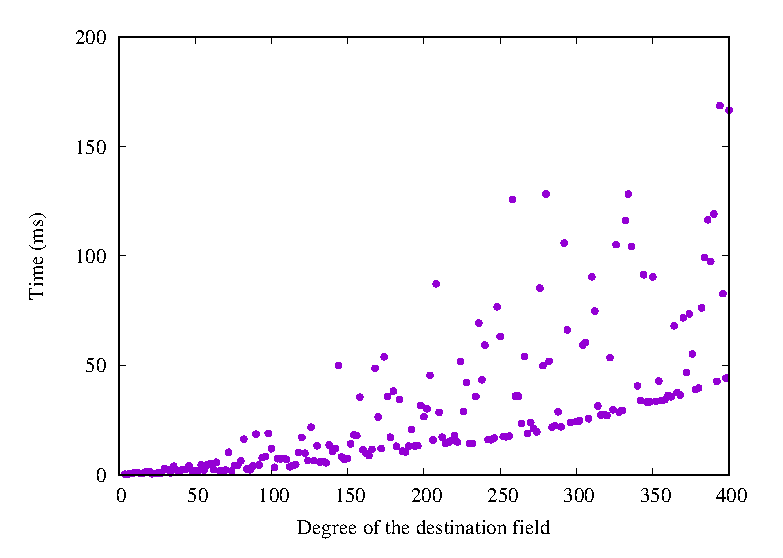
\includegraphics{benchmarks/lattice-bcs/embed-from-2-up-3.eps}
  \caption{Timings for the computation of embeddings from $\mathbb{F}_{p^{2}}$
  to $\mathbb{F}_{p^{m}}$ for $m\leq 400$ and $2\mid m$, with $p=3$. The
  embeddings were computed with increasing degrees.}
  \label{fig:bcs-embed-from-2-up}
\end{figure}
When the embeddings are computed with decreasing degrees, there are a lot more
embeddings already in the lattice, thus the defect can be either $1$ or $2$. We
observe that the time needed to compute the embeddings is completely different
in those two cases, thus we use a logarithmic scale to emphasize the difference.
\begin{figure}
  \centering
  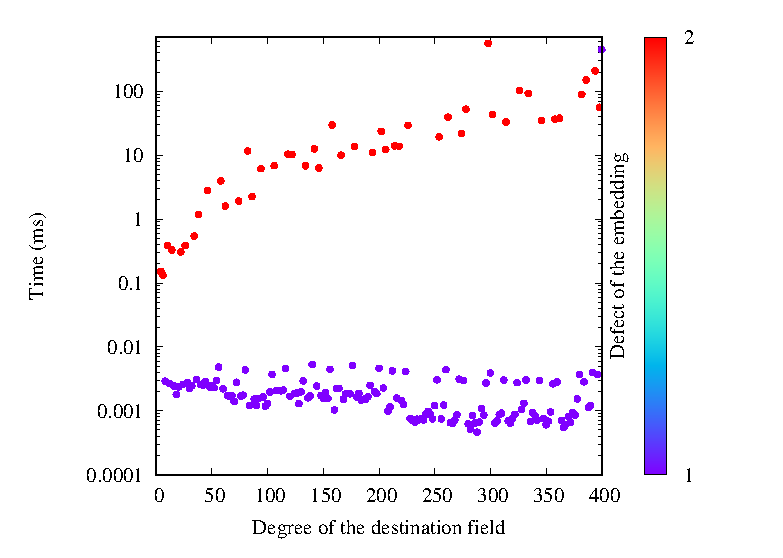
\includegraphics{benchmarks/lattice-bcs/embed-from-2-down-3.eps}
  \caption{Timings (logarithmic scale) for the computation of embeddings from
    $\mathbb{F}_{p^{2}}$ to $\mathbb{F}_{p^{m}}$ for $m\leq 400$ and $2\mid m$,
  with $p=3$. The embeddings were computed with decreasing degrees.}
  \label{fig:bcs-embed-from-2-down}
\end{figure}
The difference between the two methods is also noticeable when looking at the
embeddings to a fixed finite field. We look at the embeddings to the finite
fields of degree $360$ because it is a highly composite number, having $24$
different divisors: $1, 2, 3, 4, 5, 6, 8, 9, 10, 12, 15, 18, 20, 24, 30, 36, 40,
45, 60, 72, 90, 120, 180$ and $360$. In the first experiment, with increasing
degrees, all embeddings are computed in under one second, as shown in
Figure~\ref{fig:bcs-embed-to-360-up}. It is understandable because the defect is
never very high. In the second experiment, shown in
Figure~\ref{fig:bcs-embed-to-360-down}, the timing to compute the embedding 
\[
  \mathbb{F}_{p^{180}}\emb\mathbb{F}_{p^{360}}
\]
is approximately $30$ seconds, with a defect of $180$ because
$\mathbb{F}_{p^{360}}$ has no embedded subfields yet. After this computation,
only the embedding $\mathbb{F}_{p^{120}}\emb\mathbb{F}_{p^{360}}$ has a defect
equal to $2$ and all the others have a defect equal to $1$. This leads to very
fast computation for some embeddings, that are essentially already computed.
\begin{figure}
  \centering
  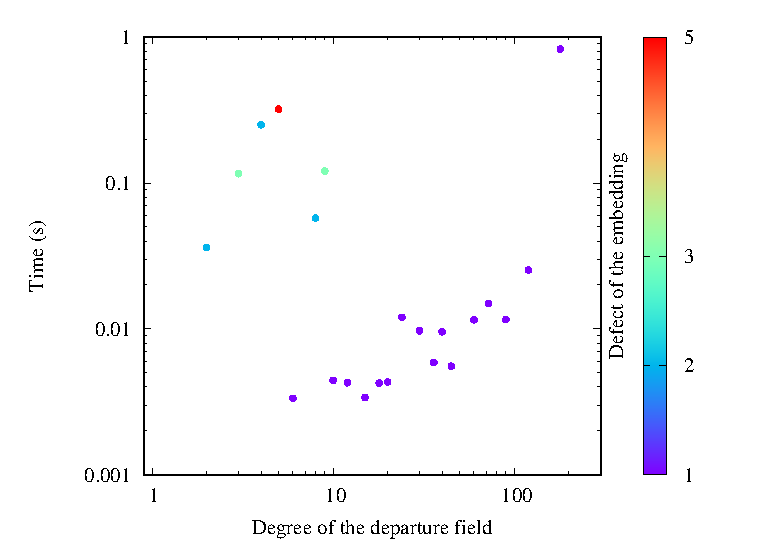
\includegraphics{benchmarks/lattice-bcs/embed-to-360-up-3.eps}
  \caption{Timings for the computation of embeddings from $\mathbb{F}_{p^{m}}$
  to $\mathbb{F}_{p^{360}}$ for $m\mid 360$, with $p=3$. The
  embeddings were computed with increasing degrees. We use logarithmic scales on
  both axes for readability.}
  \label{fig:bcs-embed-to-360-up}
\end{figure}
\begin{figure}
  \centering
  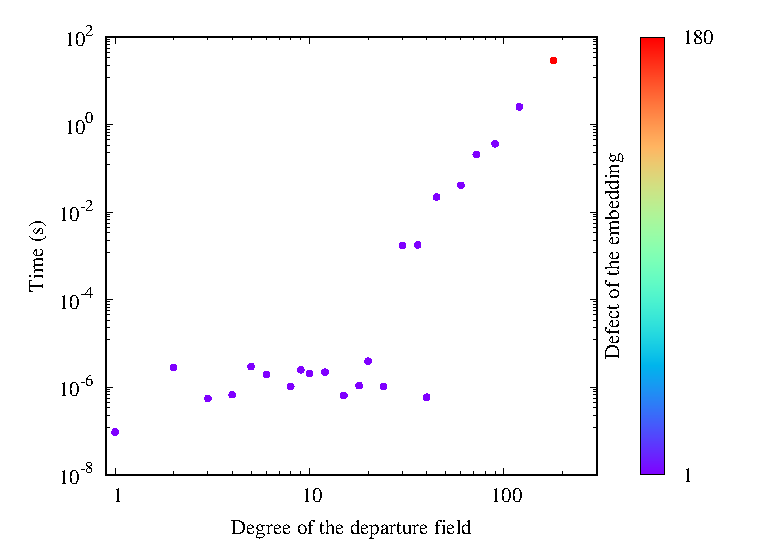
\includegraphics{benchmarks/lattice-bcs/embed-to-360-down-3.eps}
  \caption{Timings for the computation of embeddings from $\mathbb{F}_{p^{m}}$
  to $\mathbb{F}_{p^{360}}$ for $m\mid 360$, with $p=3$. The
  embeddings were computed with decreasing degrees. We use logarithmic scales on
  both axes for readability.}
  \label{fig:bcs-embed-to-360-down}
\end{figure}
When computing embeddings corresponding to extension of a fixed degree, \eg
extensions of type
\[
  \mathbb{F}_{p^{2m}}/\mathbb{F}_{p^{m}},
\]
the difference is also noteworthy: when the embeddings are computed with the
degrees decreasing (Figure~\ref{fig:bcs-embed-fixed-degree-down}), then the defect is
always maximum, thus the timings are rather smooth, while the computations with
the increasing degrees (Figure~\ref{fig:bcs-embed-fixed-degree-up}) produce
erratic timings because low defects lead to a huge speedup.
\begin{figure}
  \centering
  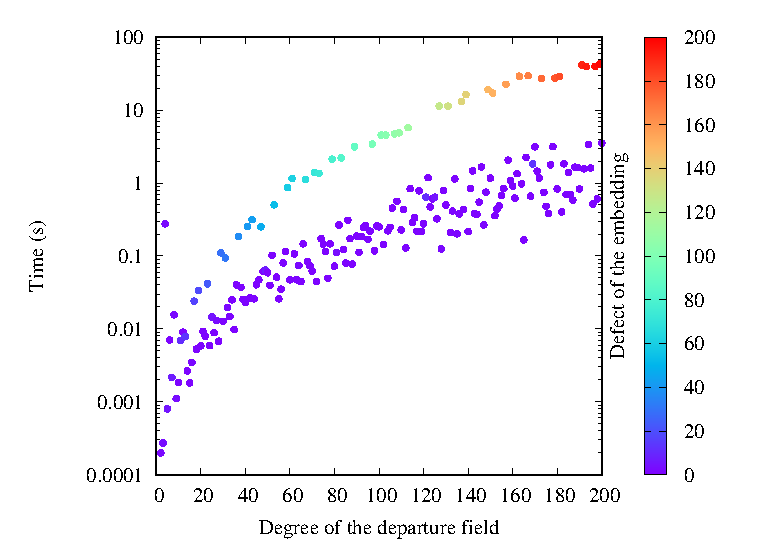
\includegraphics{benchmarks/lattice-bcs/embed-fixed-degree-from-12-to-24-up.eps}
  \caption{Timings (logarithmic scale) for the computation of embeddings from $\mathbb{F}_{p^{m}}$
  to $\mathbb{F}_{p^{2m}}$ for $1\leq m\leq 200$, with $p=3$. The
  embeddings were computed with increasing degrees.}
  \label{fig:bcs-embed-fixed-degree-up}
\end{figure}
\begin{figure}
  \centering
  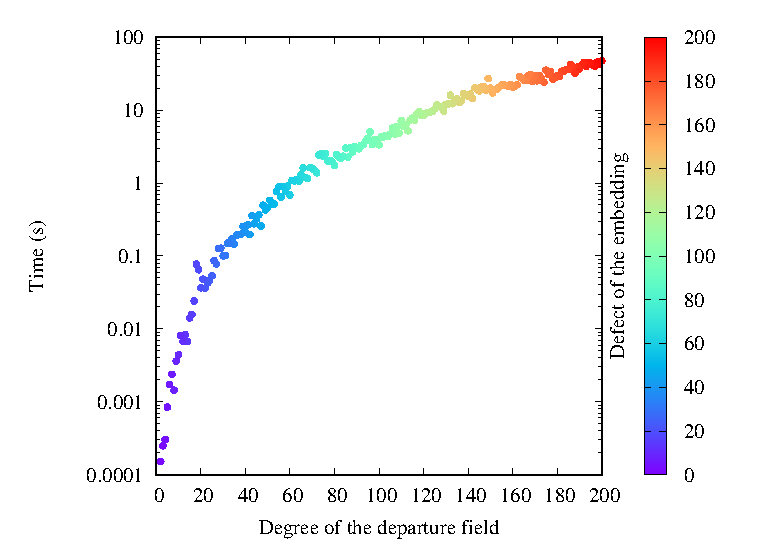
\includegraphics{benchmarks/lattice-bcs/embed-fixed-degree-from-12-to-24-down.eps}
  \caption{Timings (logarithmic scale) for the computation of embeddings from $\mathbb{F}_{p^{m}}$
  to $\mathbb{F}_{p^{2m}}$ for $1\leq m\leq 200$, with $p=3$. The
  embeddings were computed with decreasing degrees.}
  \label{fig:bcs-embed-fixed-degree-down}
\end{figure}
In order to show the impact on the characteristic $p$ on the timings, we also
plot the time needed to compute the embedding
\[
  \mathbb{F}_{p^{12}}\emb\mathbb{F}_{p^{24}}
\]
for different primes $p$. Because the impact on the timing is logarithmic in the
characteristic $p$, we use each the prime numbers found immediately after $2^j$,
for $1\leq j\leq m$, \ie $p\approx 2^j$. The result is shown in
Figure~\ref{fig:bcs-embed-primes}.
\begin{figure}
  \centering
  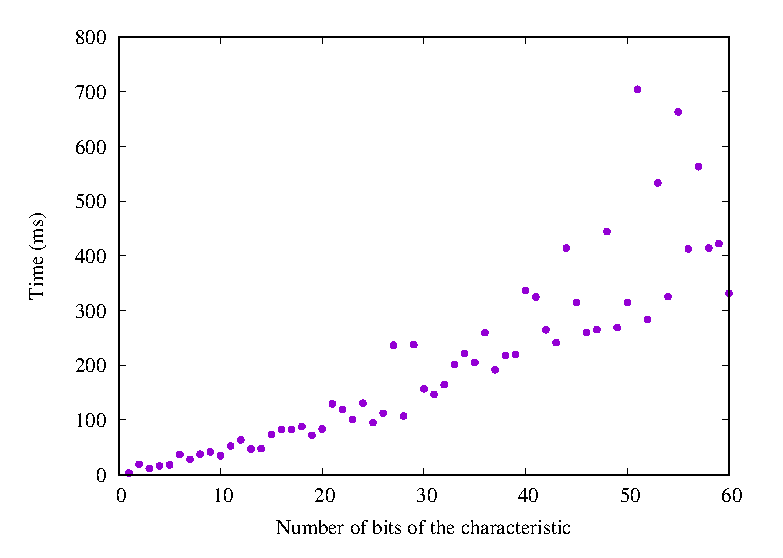
\includegraphics{benchmarks/lattice-bcs/embed-primes-exp.eps}
  \caption{Timings for the computation of embeddings from $\mathbb{F}_{p^{12}}$
  to $\mathbb{F}_{p^{24}}$ with $p$ a prime number growing up to approximately
  $2^{60}$.}
  \label{fig:bcs-embed-primes}
\end{figure}
Whether or not compatibility conditions have to be fufilled when computing an
embedding implies different internal routines in Bosma-Canon-Steel framework,
such as intersections computations and reccursive computations of other
embeddings. However, the different possible scenarios share the preponderance of the
root finding in the timings: it is the critical routine in all cases. Although,
for embeddings involving small degree finite fields and with a low defect (\ie
when other embeddings have already been computed and information is known) the
time spent dealing with high level routines can be substantial. It is not
really a problem because in that case the computations are very fast, but it
indicates that the julia code could be optimized some more.

% TODO
% ====
%
% Comparison with MAGMA? Critical routines!
%%
